\documentclass[10pt,letterpaper]{article} 

\usepackage{multirow}
\usepackage{cogsci} 
\usepackage{pslatex} 
\usepackage{graphicx}
\usepackage{pdfsync}
\usepackage{apacite}
\usepackage[raggedright]{sidecap}


\title{Developmental and postural changes in children's visual access to faces}

% \author{{\large \bf Michael C. Frank} \\ \texttt{mcfrank@stanford.edu} \\ Department of Psychology \\ Stanford University \And
% {\large \bf Kaia Simmons} \\ \texttt{kaias@stanford.edu} \\ Program in Human Biology \\ Stanford University 
% \And {\large \bf Daniel Yurovsky} \\ \texttt{dyurovsky@stanford.edu} \\ Department of Psychology \\ Stanford University
% \And {\large \bf Guido Pusiol} \\ \texttt{pusiol@stanford.edu} \\ Department of Psychology \\ Stanford University}

\author{{\large \bf Michael C. Frank, Kaia Simmons, Daniel Yurovsky, \& Guido Pusiol} \\
\texttt{\{mcfrank,kaias,yurovsky,pusiol\}@stanford.edu} \\
Department of Psychology \\
Stanford University}

\begin{document}

\maketitle

\begin{abstract} 

The faces of other people are a critical information source for young children. During early development, children undergo significant postural and locomotor development, changing from lying and sitting infants to toddlers who walk independently. We used a head-mounted camera in conjunction with a face-detection system to explore the effects of these changes on children's visual access to their caregivers' faces during an in-lab play session. In a cross-sectional sample of 4--20 month old children, we found substantial changes in face accessibility based on age and posture. These changes may translate into changes in the accessibility of social information during language learning. 

{Keywords:} Social development; face processing; head-camera.
\end{abstract}

\section{Introduction}

A father offers his young daughter a novel object: a bright yellow feather duster. A few moments after she accepts the toy, he remarks, ``Isn't the zem funny?'' Her father may still be talking about the feather duster, or he may be describing a new object.  To find out she has access to a simple and reliable method: she can look to his face to infer the direction of his attention. 

The ability to follow social signals like eye-gaze is an important part of early social cognition \cite{scaife1975} and a strong predictor of children's early language development. For example, \citeA{brooks2005} found that children who followed an experimenter's gaze better before their first birthday had larger vocabularies at 18 months. Similarly, \citeA{carpenter1998} found that children's level of joint engagement (as well as the degree to which mothers followed the child's focus of attention in their labeling) predicted vocabulary growth in both language production and comprehension. These studies suggest that children's social environment plays a powerful supportive role in language learning. 

But at the same time as children are beginning to learn their first words, their view of the world is changing radically \cite{adolph2007}. As speechless infants, they are unable to locomote independently. Before their first birthday, they begin crawling; soon after, they begin to walk independently. Infants' visual field is subject to the whims of their caregivers, but caregivers often place them in positions conducive to joint attention. In contrast, toddlers determine their own input to a much greater degree, but as a consequence they spend much of their time in a world primarily populated by knees. These postural and locomotor changes may have a profound effect on what children see.

A recent study suggests the possibility of links between motor milestones, social cognition, and language. \citeA{walleunderreview} noted robust correlations between children's ability to walk and their vocabulary, both receptive and productive. On the basis of an observational study of parent input, they speculated that the emergence of walking may change the ability of the child to access social information (because walking toddlers see more of the social world than crawling infants). Accessing more social information may in turn allow children to discover word meanings more effectively.

Recent methodological developments have the potential to provide data that would allow this hypothesis to be tested. The availability of head-mounted cameras and eye-trackers allows for the measurement of children's naturalistic environment in a way that was not previously possible. \citeA{yoshida2008} gave the first demonstration of the radical differences between toddler and adult perspectives on the social world, with toddlers' visual field being dominated by hands and objects much more than that of adults. More recent work has used head-mounted eye-tracking methods to measure young toddlers' fixations \cite{franchak2011}, also finding that children look relatively infrequently at their mothers' faces in naturalistic play.

These methods are now being applied to understand inputs to language acquisition. Work by Yu, Smith, and colleagues suggests that word learning is facilitated when parents and children create moments in which the visual field is dominated by a single object \cite{smith2011,yuinpress}. Some data even suggest that young children's restricted viewpoint may be more effective for learning words than the comparable adult perspective \cite{yurovsky2012}. Together, this body of evidence suggests that measuring infants' perspective---and how it changes in motor development---is a critical part of understanding early language learning.

In the current study we took a developmental approach to understanding the relationship between perspective and access to social information. We recorded head-camera data from a group of infants and children across a broad age range as they played with their caregivers during a brief laboratory visit. We then hand-annotated these data for the child's posture and parents' naming behavior and used face-detection algorithms to measure the frequency of faces in the child's visual field.  The resulting dataset allows us to analyze changes in access to faces according to children's age, posture, and linguistic input. 

\section{Methods}

\subsection{Participants}

Participants were 20 infants and children (N=4 each at 4, 8, 12, 16, and 20 months, 9 females total) in an ongoing large-scale study, recruited from the surrounding community via state birth records. Participants had no documented disabilities and were reported to hear at least 80\% English at home. Success rates for children wearing the camera for long enough to initiate the play session varied from 100\% at 8 months to approximately 50\% at 20 months. 

% The participants in our study are twenty infants whom we invited to the Social Cognition lab for hour-long sessions. The infants fall into five age groups (with four infants in each group): 4-, 8-, 12-, 16-, and 20-month-olds. Using the Center for Infant Studies (CIS) database, we screen for participants who are in the appropriate age ranges and have no documented developmental disabilities.

\subsection{Head-mounted camera}

\begin{figure}
\centering
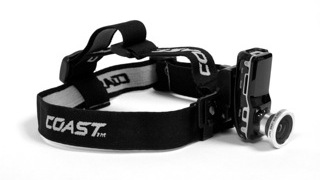
\includegraphics[width=2in]{figures/headcam_w_fisheye3.jpg}
\caption{\label{fig:headcam} Our light-weight, low-cost head-mounted camera with fisheye lens.} 
\end{figure}

Our head-mounted camera (``headcam'') is composed of a small, inexpensive MD80 model camera attached to a soft elastic headband from a camping headlamp. An aftermarket fisheye lens intended for iPhones and other Apple devices is attached to increase view angle. The total cost of each camera is approximately \$60. The camera captures 720x480 pixel images at approx. 25 frames per second, and has battery life of 60--90 minutes. Without the fisheye lens, the viewing angle for the camera is $32^{\circ}$ horizontal by $24^{\circ}$ vertical; with the fisheye, $64^{\circ}$ horizontal by $46^{\circ}$ vertical. The device is pictured in Figure \ref{fig:headcam}.

The vertical field of view of the camera was considerably smaller than the child's approximate vertical field of view, which---even at 6-7 months---spans around 100--120$^{\circ}$ in the vertical dimension \cite{mayer1988,cummings1988}. We were therefore faced with a choice in the orientation of the camera. If we chose a lower or higher orientation, we would be at risk of truncating either the child's own hands and physically proximate objects, or the faces of the adults around the child. Yet if we chose the middle orientation, we would still be at risk of underestimating the proportion of faces viewed by the child. Thus, for the purposes of the current study---measuring visual access to faces---we chose to orient the camera towards the upper part of the visual field.\footnote{Previous studies have shown that children's head movements in the horizontal dimension are approximated by (though are slightly lagged by) their head movements \cite{yoshida2008}. Our own experience with the current apparatus ratifies these conclusions for the horizontal field but suggests that head movements in the vertical field are less reliable. Hence, these studies may run the risk of underestimating the proportion of faces actually seen by children.} While this orientation decreased our chances of recording the objects being manipulated by the child, it nevertheless allowed us to capture the majority of the faces in the child's visual field.

\subsection{Procedure}

After coming to the lab, families were seated in our waiting room where they signed consent documents and where children were fitted with the headcam. After a short period of play, they were escorted to a playroom in the lab where the free-play session (the focus of the current study) was conducted. 

In the waiting room, the experimenter placed the headcam on children's heads after they had time to adjust to the environment. For children who resisted wearing the headcam, the experimenter used distractor techniques (presenting stimulating toys or engaging the children in hand-occupying activities) intended to keep children's focus elsewhere and prevent them from taking off the camera \cite{yoshida2008}. Once the child was wearing the camera comfortably for a period of time, child and caregiver (or caregivers: in two cases, there were two adults present) were escorted to the playroom. 

In the playroom, the experimenter presented the child's parent with a box containing three labeled pairs of objects, each consisting of a familiar and a novel object (e.g. a ball and a feather duster, marked as a ``zem''). Parents confirmed that the child had not previously seen the novel toys. Parents were instructed to play with the object pairs with the child, one at a time, ``as they typically would'' and to use the novel labels to refer to the three toys. After giving these instructions, the experimenter left the room for a period of approximately 15 minutes. During this time, a tripod-mounted camera recorded video from a corner of the room and the headcam captured video from the child's perspective. 

\subsection{Data Processing and Annotation}

\begin{figure*}
\includegraphics[width=7in]{figures/framesample.pdf}
\caption{\label{fig:frames} Sample frames from the headcam videos for a child from each age group, selected because they featured successful face detections (green squares).} 
\end{figure*}

All headcam videos were cropped to exclude the period of entry to the playroom and were automatically synchronized with the tripod-mounted videos using FinalCut Pro Software. The final sample was approx. 5 hours of headcam video (M = 12 min, range: 2--21 min), for a total of roughly 400,000 frames. 

\subsubsection{Posture and Orientation Annotation}

One major goal of our study was to understand the relationship between children's posture and their access to information from the faces of their caregiver. To investigate this relationship, we created a set of annotations for the child's physical posture (e.g. standing, sitting) and orientation of the caregiver relative to the child (e.g. in front of, behind, close, far away). For each headcam video, a coder used OpenSHAPA software to annotate both orientation and posture \cite{adolph2012}. 

Orientation was initially categorized as having the caregiver in front, to the side, or behind the child, and close (defined informally as within arm's reach) or farther away. Because of data sparsity, we consolidated this scheme into three categories: close to the caregiver with the caregiver either in front or on the side, farther from the caregiver again with caregiver either in front or on the side, and a global category of caregiver behind the child. Posture was categorized as being held/carried, lying face-up, sitting, prone (crawling or lying), standing, or other. Data from when the child was out of view of the tripod camera was marked as uncodable and excluded from these annotations. 
% A second coder coded XYZ videos; their categorizations were reliable at XYZ. 

\subsubsection{Labeling Annotation}

We were also interested in the availability of social information proximate to naming events in the caregivers' speech to children. Accordingly, a human coder marked the onset time when the name of any of the six objects in the object set was used. Overall, caregivers produced a median of 35 labels in a highly skewed distribution across participants (range: 9 -- 131).

\subsection{Face Detection}

An additional goal of the study was to measure the presence of caregivers' faces in the child's field of view (as approximated by the headcam). To avoid hand-annotating the size and position of faces in every frame of video, we tested two face detection systems. Sample frames from the video with successful detections are given in Figure \ref{fig:frames}.

\subsubsection{Face detection algorithms}

The first algorithm was based on freely available computer vision tools \cite{bradski2008} and is described in depth in our previous work \cite{frank2012b}. This system had two parts. The first was the application of a set of four Haar-style face detection filters \cite{viola2004} to each frame of the videos independently. These detectors each provide information about whether a face is present in the frame as well as size and position for any detections. In a second step, these detections are then combined via a hidden Markov model (HMM), trained on hand-annotated data (see Appendix). The HMM model (which performed nearly as well as the more complex and computationally-intensive Conditional Random Field model used in our previous work) attempted to estimate whether a face was truly present in each frame of the videos, using as its input the number of Haar detectors that were active in any given frame. 

The second algorithm that we evaluated was a semi-automated adaptive tracker-by-detection (SAATD). The algorithm required manual user input (selecting a single face example per video) for its initialization, but then needed no additional training data. The tracker is based on \citeA{kalal2010} which uses patches in the trajectory of an optical-flow based tracker \cite{lucas1981} to train and update a face detector. The optical flow tracker and the face detector work in parallel. 
% For detection, we keep positive and negative templates of previously detected faces. 
If the face detector finds a location in a new frame exhibiting a high similarity to its stored template, the tracker is re-initialised on that location. Otherwise, the tracker uses the optical flow to decide the location of a face in the new frame.
 % The face detector is trained using visual features \cite{lepetit2005} and the detection is performed using a random ferns classifier \cite{ozuysal2007}. 
The primary advantage of the SAATD algorithm is the use of motion for face detection: Following the movement of the pixels that define a face it is possible for the algorithm to adapt to new morphologies (i.e. different face poses). 
%One disadvantage, however, is the necessity of manual initialization.


% [1] Z. Kalal, J. Matas, and K. Mikolajczyk. P-N learning: Bootstrapping binary classifiers by structural constraints. In 2010 IEEE Conference on Computer Vision and Pattern Recognition (CVPR), pages 49–56. IEEE, June 2010.


% [2] B. D. Lucas and T. Kanade. An iterative image registration technique with an application to stereo vision. In Proceedings of the International Joint Conference on Artificial Intelligence, pages 674–679, 1981


% [3] V. Lepetit, P. Lagger, and P. Fua. Randomized trees for Real-Time keypoint recognition.
% In IEEE Computer Society Conference on Computer Vision and Pattern Recognition, volume 2, pages 775–781, Los Alamitos, CA, USA, 2005. IEEE Computer Society.

% [4] M. Ozuysal, P. Fua, and V. Lepetit. Fast keypoint recognition in ten lines of code. In IEEE Conference on Computer Vision and Pattern Recognition, Los Alamitos, CA, USA, June 2007. IEEE.




\begin{figure*}[t]
\centering
\includegraphics[width=3in]{figures/posture.pdf}
\includegraphics[width=3in]{figures/orientation.pdf}
\caption{\label{fig:posture} Proportion time in each posture, plotted by child's age (left panel). Proportion time in each orientation relative to the caregiver, again plotted by child's age (right panel). For clarity, the ``other'' code is not plotted in either figure. Error bars show standard error of the mean across participants.} 
\end{figure*}


\subsubsection{Detector evaluation}

To ensure that our evaluation was not biased by the relatively rare appearance of faces in the dataset, we annotated two samples, both a random sample from the data and a sample with a high-density of faces (see Appendix). We evaluated each algorithm on its precision (hits / hits + false alarms) and recall (hits / hits + misses), as well as F-score (the harmonic mean of these two measures). Results are reported in Table \ref{tab:results}. 

The HMM model obtained a relatively high level of performance for the random subsections, but performed poorly when there was a relatively high density of faces present. In contrast, SAATD performed well on both samples, giving better performance especially in cases where there was partial occlusion. Our goal in using face-detection algorithms was to provide a measurement technique that eliminated tedious and expensive hand-coding and provided acceptable results. We therefore selected the SAATD model and report detections from this algorithm as an estimate of face presence in all further analyses. 

\begin{table}[t]
  \caption{Model performance on gold standard generalization training set dataset. P, R, and F denote precision, recall, and F-score for each of the two samples. \label{tab:results} } 
  \begin{center} 
    \begin{tabular}{l|ccc|ccc} 
      \hline
       &  \multicolumn{3}{c|}{High-density} &  \multicolumn{3}{c}{Random} \\
      \null Model & P & R & F & P & R & F  \\ 
      \hline 
      HMM &.55  & .38 &  .45 & .89 & .74 & .81   \\
      SAATD & .86 & .78 & .81 & .93 & .76 & .83 \\      
    \hline 
    \end{tabular} 
  \end{center}
\end{table}



\section{Results}

We report results from three different sets of analyses. First, we explore developmental changes in posture and orientation in our dataset. Next, we explore how these changes affect access to faces, as measured using our face-detection algorithm. Finally, we report preliminary results on the accessibility of faces during labeling.

\subsection{Changes in Posture and Orientation}
 
Our posture coding captured typical developmental milestones (Figure \ref{fig:posture}, left). Overall, sitting was the most common posture for interactions in the caregiver play session. The youngest infants in our sample mostly sat (with parental assistance), but also lay down and were carried a significant proportion of the time. The 12-month-olds were the only group who spent a large amount of time crawling, and the 16- and 20-month-olds sat and stood in equal parts. 

Similarly, our coding of orientation revealed some significant developmental changes (Figure \ref{fig:posture}, right). Younger children more frequently had the caregiver behind them, often because the caregiver was supporting the child's sitting posture (for the 4-month-olds especially). In contrast, the 12--20 month olds were able to locomote independently and so were able to spend more time further from the caregiver. 


\begin{figure*}[t]
\includegraphics[width=2.3in]{figures/prop_faces_age.pdf}
\includegraphics[width=2.3in]{figures/prop_faces_posture.pdf}
\includegraphics[width=2.3in]{figures/prop_faces_orientation.pdf}
\caption{\label{fig:face_dets} Proportion face detections, split by age group (left panel), posture (middle panel), and caregiver's orientation (right panel). We omit the lying face-up posture due to data sparsity. Black points show individual participants and are jittered slightly on the horizontal, red lines show means and 95\% confidence intervals.} 
\end{figure*}


\subsection{Access to Faces }

We next investigated the effects of the child's posture and orientation on the presence and size of the caregiver's face in the visual field. Figure \ref{fig:face_dets} shows the proportion of frames with a positive face detection, plotted by the child's age, posture, and orientation relative to the caregiver. 

Overall, there were very large differences in access to faces across age. The 4-month-olds saw almost no faces---their parents were behind them most of the time, supporting them since they could not sit independently. In contrast, the 8-month-olds, who could sit independently, typically sat across from their caregiver and saw many faces in both the sitting and prone postures. The 12-month-olds spent a large amount of time in the prone position (typically crawling after the ball, for example) and saw almost no faces in that posture. The 16- and 20-month-olds saw many faces because they were standing while their parents were sitting, putting their faces at a relatively similar level.

Across ages, the carrying and prone postures resulted in the smallest number of faces seen, while standing and sitting resulted in far more. These postures both presented opportunities for seeing faces in large part because parents were sitting or lying on the floor with children. Although far fewer faces were seen when the caregiver was behind the child,\footnote{Since orientation was coded via body posture, faces seen while the caregiver was behind the child were due to children looking over their shoulder.} both the close and far positions resulted in approximately equal proportions of face detections. 

\subsection{Access to Faces During Labeling}

Our final analysis concerned the accessibility of caregivers' faces during labeling events. \citeA{franchak2011} found that referential speech was marginally more likely to draw toddlers' attention to mothers' faces. We were similarly interested in whether looking at faces occurred during labeling. Accordingly, we used the labeling annotations for each child to identify the 2s before and after each labeling event. We then computed the proportion face detections within this window across ages. 

The overall pattern of face accessibility closely mirrored the base rates shown in Figure \ref{fig:face_dets}. Although this general pattern in itself is important in assessing developmental access to social information, in the current analysis we were interested in whether there was differential access to faces around labeling instances. We thus computed difference scores between the baseline face detection rate and the rate of face detections in labeling windows for each participant. Figure \ref{fig:naming_face} shows the results of this analysis. 

Although any conclusion must remain extremely tentative because of the small sample, we nevertheless saw an increase in label-related face access for the 20-month-olds. This difference was robust across a variety of window sizes from 1--6 s. (8-month-olds were more variable but similarly showed some trend towards greater face access during naming.) We cannot yet make inferences about the source of these differences: They could be could be caused by children, caregivers, or a combination of the two. Nevertheless, these results converge with previous work and suggest that, in combination with face detection techniques, the headcam may be a viable method for examining social access during language learning.

\begin{figure}
\begin{center}
  \includegraphics[width=3in]{figures/naming_faces_diff.pdf}
\end{center}
\caption{\label{fig:naming_face} Proportion of faces detected in a 4s window of time centered around labeling events, plotted by age group and whether the word was familiar or novel. Error bars show 95\% confidence intervals. 4-month-olds are omitted due to the limited number of total face detections for this group.} 
% \vspace{-ex}
\end{figure}

\section{General Discussion}

Using a head-mounted camera, we explored the relationship between infants' postural and locomotor development and their visual access to social information. The use of automated annotation tools from computer vision allowed us to measure the prevalence of caregivers' faces in their children's visual field. We found systematic differences in the visual accessibility of faces based on posture, orientation, and age, as well as hints of differences in language-related changes in visual access. While these results remain preliminary given the size of our developmental sample, this work nevertheless provides an important proof-of-concept that computer vision techniques can be used as a measurement method in the developmental context. 

The measures developed here have broad applicability to the study of individual and cultural differences. Since the physical circumstances of child rearing vary widely across households and across cultures, there may be important and predictable differences in children's visual experience. As suggested by the correlations between walking and vocabulary development \cite{walleunderreview}, postural development may have substantial downstream consequences for language. For example, shifts in how infants are placed in particular postures by strollers or carriers \cite{zeedyk2008} or how their motor development is encouraged by parent practices \cite{bril1986} may lead to differences in social input which in turn affect their language learning. Since our variant of the headcam method is both inexpensive and highly portable, we have been able to deploy it in children's homes with some success; it may thus be a valuable tool for investigating differences in child-rearing practices.

A deep body of work uses children's linguistic input---measured using audio recordings---to understand the learning mechanisms underlying vocabulary acquisition \cite{huttenlocher1991,hart1995,fernald2006}. There have been some important initial successes in using visual input to predict language uptake \cite{yuinpress}. Nevertheless, we have a long way to go before our knowledge about children's visual input parallels our understanding of their linguistic environment. Coming to such an understanding will require the creation of both corpus resources and automated tools such as those we have begun to develop here.


\section{Acknowledgments}

Thanks to Ally Kraus, Kathy Woo, Aditi Maliwal, and other members of the Language and Cognition Lab for help in recruitment, data collection, and annotation. This research was supported by a John Merck Scholars grant to MCF.

\bibliographystyle{apacite}

\setlength{\bibleftmargin}{.125in} \setlength{\bibindent}{-\bibleftmargin}

\bibliography{postureface.bib}

\section{Appendix: Face presence annotation}

We selected 1 minute of interaction for each age group, divided evenly across the four dyads at that age. For each dyad, we divided the recorded video into contiguous 1 s segments and selected 16 in accordance with two criteria. First, 8 of these segments were selected by choosing the parts of the videos highest in face detection (\emph{high density sample}). To be fair to both algorithms, half of this was chosen from the segments with the most HMM detections and half were chosen from the segments with the most SAATD detections. The remaining segments were chosen by randomly sampling from segments not yet selected for coding (\emph{random sample}). 
% This scheme was chosen to ensure selection of a representative sample from the interactions. 
Segments were annotated frame-by-frame by a human coder, who marked each frame as containing a face if at least half of the face was in the child's view. Detector output for each of these frames was then compared to this gold standard. A detection was counted as correct if it overlapped a face with half of its total area. The HMM training sample was selected via the same method as this gold standard sample, but used separate set of video segments.

% This liberal criterion was adopted because the field of view of the camera was known to be smaller than the field of view for the children in our sample. 

\end{document}

